\documentclass[11pt]{scrartcl}
\usepackage[dvipsnames,svgnames]{xcolor}
\usepackage{tikz}
\usetikzlibrary{shapes,decorations.shapes}
\newsavebox{\mycandle}
\savebox{\mycandle}{
	
\begin{tikzpicture}[scale=.1]
		\shade[top color=yellow,bottom color=red] (0,0) .. controls (1,.2) and (1,.5) .. (0,2) .. controls (-1,.5)  and  (-1,.2) .. (0,0);
		\fill[yellow!90!black] (.8,0) rectangle (-.8,-5);
	\end{tikzpicture} }

\tikzset{
	paint/.style={draw=#1!50!black, fill=#1!50},
	my star/.style={decorate,decoration={shape backgrounds,shape=star},
			star points=#1}
}

\begin{document}
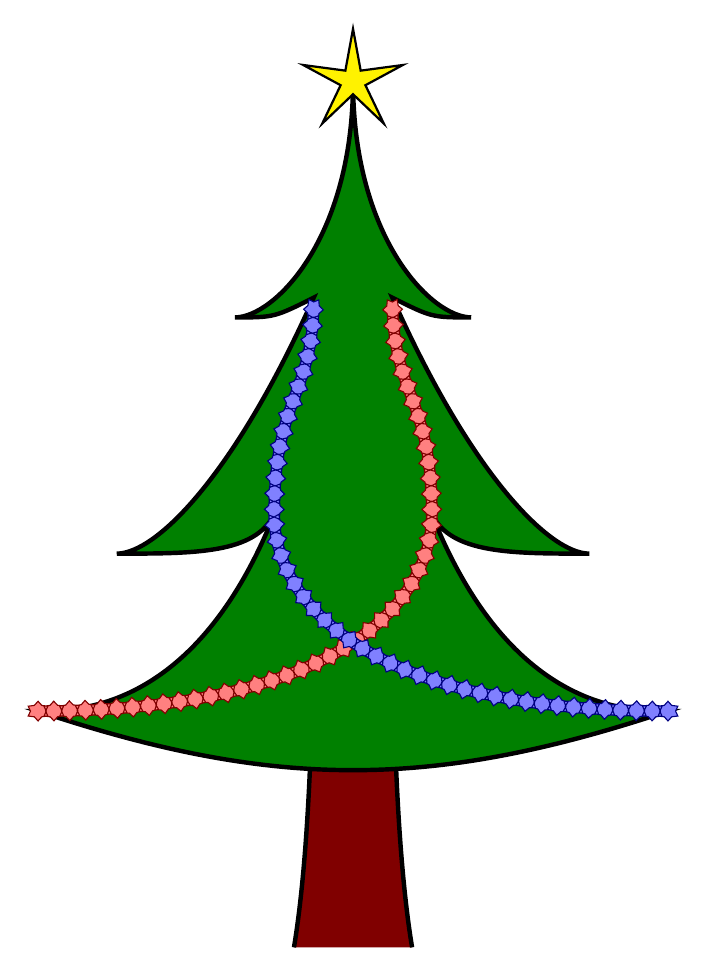
\begin{tikzpicture}
	\draw[fill=Maroon,ultra thick]
	(.75,-1)  ..  controls (.5,.5)  and   (.5,3)    .. (0.5,4)
	-- (-0.5,4)  ..  controls (-.5,3) and (-.5,.5)     .. (-.75,-1) ;
	\draw[ultra thick,fill=green!50!black]
	(0,10) .. controls  (0,8)     and   (1,7)    .. (1.5,7)
	..  controls (1,7)     and   (1,7)    .. (0.5,7.25)
	..  controls (1.5,5)   and   (2.5,4)  .. (3,4)
	..  controls (2,4)     and   (1.25,4) .. (1,4.5)
	..  controls (2,2)     and   (3.5,2)  .. (4,2)
	..  controls (1,1)     and   (-1,1)   .. (-4,2)
	..  controls (-3.5,2)  and   (-2,2)   .. (-1,4.5)
	..  controls (-1.25,4) and   (-2,4)   .. (-3,4)
	..  controls (-2.5,4)  and   (-1.5,5) .. (-0.5,7.25)
	..  controls  (-1,7)   and   (-1,7)   .. (-1.5,7)
	..  controls  (-1,7)   and   (0,8)    .. (0,10)
	;
	\foreach \candle in {(2,5),(-2,5),(0.5,7.5),(-0.5,7.5),(-3,2.5), (3,2.5),
			(1.5,1.75),(-1.5,1.75)}
	\node at \candle {\usebox{\mycandle}} ;
	\node [star, star point height=.5cm, minimum size=.5cm, draw,fill=yellow,thick]
	at (0,10) {};
	\begin{scope}[decoration={shape sep=.2cm, shape size=.25cm}]
		\draw [my star=6, paint=red]  (-4,2)
		..  controls (0,2)     and   (1,3.5)   .. (1,4.5)
		..  controls (1,6)     and   (0.5,6)      .. (0.5,7.25);
		\draw [my star=6, paint=blue]  (4,2)
		..  controls  (0,2) and (-1,3.5)      .. (-1,4.5)
		..  controls (-1,6)     and   (-0.5,6)      .. (-0.5,7.25);
	\end{scope}
\end{tikzpicture}

\end{document}
